\documentclass[a4paper,twoside,11pt,openright]{report}


\usepackage[utf8]{inputenc}
\usepackage[T1,OT2,T1]{fontenc}
\usepackage{lmodern}
\usepackage{parskip}
\usepackage{a4wide}
\usepackage{tabularx}
\usepackage{graphicx}
\usepackage{url}
\usepackage{textcomp}
\global\let\textlangle\relax
\global\let\textrangle\relax
\usepackage{textcmds}
\usepackage{units}
\usepackage{listings}
\usepackage[figuresright]{rotfloat}
\usepackage{float}
\usepackage[colorlinks]{hyperref}
%\usepackage{hyperref}
\usepackage{subfig}
\usepackage{caption}
\usepackage{afterpage}
\usepackage{amsmath}
\usepackage{amssymb}
\usepackage{bbm}
\usepackage{mathtools}
\usepackage{exscale}
\usepackage{tikz}
\usepackage{pgfplots}
\usepackage{marvosym}
\usepackage{multicol}
\usepackage{algpseudocode}
\usepackage[chapter]{algorithm}
\usepackage{paralist}
\usepackage{dcolumn}
\usepackage{dirtree}
\usepackage[english,ngerman]{babel}
\usepackage[multiple]{footmisc}
\usepackage{eurosym}
%\usepackage[switch]{lineno}
\usepackage[colorinlistoftodos,ngerman]{todonotes}



\let\origdoublepage\cleardoublepage
\newcommand{\clearemptydoublepage}{%
  \clearpage
  {\pagestyle{empty}\origdoublepage}%
}
\let\cleardoublepage\clearemptydoublepage

\floatplacement{figure}{htb}
\floatplacement{table}{htb}
\floatname{algorithm}{Algorithmus}

\captionsetup{format=hang}
\captionsetup{justification=raggedright}

\usetikzlibrary{arrows}
\usetikzlibrary{calc}
\usetikzlibrary{decorations.pathmorphing}
\usetikzlibrary{decorations.pathreplacing}
\usetikzlibrary{shapes.symbols}
\usetikzlibrary{patterns}

\bibliographystyle{alphadin}

\lstdefinestyle{smallblock}{basicstyle=\scriptsize\ttfamily,keywordstyle=\sffamily\bfseries,numbers=left,numberstyle=\scriptsize,xleftmargin=20pt,frame=leftline,breakindent=10pt}
\lstdefinestyle{block}{basicstyle=\small\ttfamily,keywordstyle=\sffamily\bfseries,numbers=left,numberstyle=\scriptsize,xleftmargin=20pt,frame=leftline,breakindent=10pt}
\lstset{basicstyle=\ttfamily,keywordstyle=\sffamily\bfseries,breaklines}

\def\UrlBreaks{\do\:\do\.\do\@\do\\\do\/\do\!\do\_\do\|\do\;\do\>\do\]%
 \do\)\do\,\do\?\do\'\do+\do\=\do\#}
\def\UrlBigBreaks{}

\pgfkeys{/pgf/number format/.cd,
  set decimal separator={{{,}}},
  set thousands separator={{{.}}}}

%\linenumbers*


\begin{document}
\pagenumbering{roman}
\pagestyle{empty}
\begingroup
%\sffamily
\begin{center}

  \vspace*{-2.0cm}
  
\includegraphics[scale=1.4]{figures/TU_Chemnitz_positiv_gruen} \\
  \hrulefill \\[1em]
  \medskip
  \par{\huge\sffamily Fakultät für Informatik}
  \medskip
  \par{\Large\sffamily Professur Datenverwaltungssysteme}

  \vspace*{1.5cm}

  \vfill

  \vspace*{.75cm}
  \par{\scalebox{1.5}{\Huge\bfseries Bachelorarbeit}}
  \vspace*{1.5cm}
  \par{\LARGE\sffamily
    Interaktive grafische Steuerung des Growing Neural Gas\par\null}
  \vspace*{0.75cm}

  \vfill
  \vfill

  \par{\large\sffamily Tobias Gall}
  \bigskip
  \par{\large\sffamily \today}

  \vfill

  \vspace*{1.5cm}
  \begin{minipage}{0.9\textwidth}
  \large\sffamily
  \begin{tabbing}
  {\bfseries Gutachter:}	\quad\=\kill
  {\bfseries Betreuer:}		\>Johannes Fliege \\
  {\bfseries Gutachter:}	\>Prof. Dr. Wolfgang Benn \\
  				\>Johannes Fliege \\
  \end{tabbing}
  \end{minipage}
\end{center}
\endgroup

\cleardoublepage
\cleardoublepage
\pagestyle{plain}
\begingroup
\vspace*{\fill}
\centerline{\Large\textbf{Aufgabenstellung}}

\bigskip
\bigskip

\begin{quote}
\begin{center}
\Large
Interaktive grafische Steuerung des Growing Neural Gas
\end{center}
\end{quote}

\bigskip

In dieser Bachelorarbeit soll ein Konzept zu interaktiven, grafikbasierten Steuerung des Growing Neural
Gas (GNG) erarbeitet und prototypisch umgesetzt werden. Der Anwender soll die einzelnen
Arbeitsschritte (Trainingsphasen) des GNG anhand einer zweidimensionalen grafischen Darstellung des
neuronalen Netzes nachvollziehen können. Die Steuerung soll Einstellmöglichkeiten für Parameter des
GNG bieten.
\vspace*{\fill}
\endgroup

\cleardoublepage
\tableofcontents
\listoftodos
%\listoffigures
%\listoftables
%\lstlistoflistings
%\chapter*{Abkürzungsverzeichnis}
%\begingroup
\newcommand{\abkskip}{0.8ex}

\begin{center}
\begin{tabularx}{\textwidth}{>{\bfseries}lX}
%ACK   & Bestätigung (Acknowledgement) \\[\abkskip]
%AP    & Access Point \\[\abkskip]
%BSS   & Basic Service Set \\[\abkskip]
%CTS   & Clear to send \\[\abkskip]
%DA    & Zieladresse (Destination Address) \\[\abkskip]
%DCF   & Verteilte Koordinierung (Distributed Coordination Function) \\[\abkskip]
%DIFS  & DCF Interframe Space \\[\abkskip]
%DS    & Distribution System \\[\abkskip]
%DSSS  & Direct Sequence Spread Spectrum \\[\abkskip]
%ESS   & Extended Service Set \\[\abkskip]
%FHSS  & Frequency Hopping Spread Spectrum \\[\abkskip]
%HPET  & High Precision Event Timer \\[\abkskip]
%IBSS  & Independent Basic Service Set \\[\abkskip]
%LLC   & Logical Link Control Layer \\[\abkskip]
%MAC   & Medienzugriffsschicht (Medium Access Control Layer) \\[\abkskip]
%MLME  & MAC Layer Management Entity \\[\abkskip]
%OFDM  & Orthogonal Frequency-Division Multiplexing \\[\abkskip]
%PCAP  & Packet Capture library \\[\abkskip]
%PCF   & Zentrale Koordinierung (Point Coordination Function) \\[\abkskip]
%PDU   & Protocol Data Unit \\[\abkskip]
%PHY   & Darstellungsschicht (Physical Layer) \\[\abkskip]
%PIFS  & PCF Interframe Space \\[\abkskip]
%PLME  & Physical Layer Management Entity \\[\abkskip]
%RA    & Empfängeradresse (Receiving Station Address) \\[\abkskip]
%RTS   & Request to send \\[\abkskip]
%RX    & Empfänger, empfangen \\[\abkskip]
%SA    & Quelladresse (Source Address) \\[\abkskip]
\end{tabularx}
\end{center}

\newpage

\begin{center}
\begin{tabularx}{\textwidth}{>{\bfseries}lX}
%SDU   & Service Data Unit \\[\abkskip]
%SIFS  & Short Interframe Space \\[\abkskip]
%TA    & Senderadresse (Transmitting Station Address) \\[\abkskip]
%TDOA  & Time Difference of Arrival \\[\abkskip]
%TOA   & Time of Arrival \\[\abkskip]
%TOF   & Time of Flight \\[\abkskip]
%TSC   & Time Stamp Counter \\[\abkskip]
%TSF   & Timing Synchronization Function \\[\abkskip]
%TX    & Sender, senden \\[\abkskip]
%VIF   & Virtual Interface \\[\abkskip]
\end{tabularx}
\end{center}
\endgroup

%\chapter*{Symbole und Bezeichner}
%\begin{center}
\begin{tabularx}{\textwidth}{lX}
%\(c, \varepsilon, \mu\)       & Lichtgeschwindigkeit, Permittivität und Permeabilität eines Mediums        \\
%\(c_0, \varepsilon_0, \mu_0\) & \(c, \varepsilon\) und \(\mu\) im Vakuum                                   \\
%\(n = c_0 / c\)               & Brechungsindex eines Mediums                                               \\
%\(\lambda\)                   & Wellenlänge                                                                \\
%\(r, d\)                      & geometrischer Abstand                                                      \\
%\(\vec{r}\)                   & Ortsvektor in Bezug auf ein Koordinatensystem                              \\
%\(\|\vec{r}\|\)               & euklidsche Norm von \(\vec{r}\)                                            \\
%\(x, y, z\)                   & Komponenten eines dreidimensionalen Vektors                                \\
%\(t\)                         & Signallaufzeit                                                             \\[2ex]

%\(L\)                         & Länge einer IEEE 802.11 MAC-PDU in Bits                                    \\
%\(R\)                         & IEEE 802.11 Datenrate in \(\unit{MBit/s}\)                                 \\[2ex]

%\(A\)                         & Station, die eine Laufzeitmessung auslöst                                  \\
%\(B\)                         & Station, die auf \(A\) antwortet                                           \\
%\(M\)                         & Station, die den Informationsaustausch zwischen \(A\) und \(B\) beobachtet \\
%\(r_{X,Y}\)                   & Entfernung zwischen den Stationen \(X\) und \(Y\)                          \\
%\(t_{X,Y}\)                   & Signallaufzeit zwischen den Stationen \(X\) und \(Y\)                      \\[2ex]

%\(d\)                         & Übertragungsdauer eines IEEE 802.11 Frames                                 \\
%\(g\)                         & Zeit zwischen Anfrage und Antwort einer Frame-Sequenz                      \\
%\(\Delta\)                    & Gesamtdauer eines Time-of-Flight-Verfahrens                                \\
%\(T\)                         & Ereignis bzw. dessen Globalzeit                                            \\
%\(\widetilde{T}\)             & Der Zeitstempel einer Uhr bei Eintreten von \(T\)                          \\
%\(\widetilde{\Delta}\)        & Die Zeitstempeldifferenz der Ereignisse, die \(\Delta\) festlegen          \\
%\(\widehat{\Delta}\)          & Eine Schätzung für \(\Delta\) basierend auf \(\widetilde{\Delta}\)         \\[2ex]

%\(E[X]\)                      & Erwartungswert der Zufallsgröße \(X\)                                      \\
%\(D^2[X]\)                    & Varianz der Zufallsgröße \(X\)                                             \\
%\(\mu\)                       & empirischer Mittelwert einer Stichprobe                                    \\
%\(\sigma\)                    & empirische Standardabweichung einer Stichprobe                             \\
%\(\lfloor x\rfloor\)          & \(x\) ganzzahlig abgerundet                                                \\
%\(\lceil x\rceil\)            & \(x\) ganzzahlig aufgerundet                                               \\
%\(\langle x\rangle\)          & Nachkommaanteil von \(x\)                                                  \\
\end{tabularx}
\end{center}

\cleardoublepage
\setcounter{page}{1}
\pagenumbering{arabic}

\chapter{Einleitung}
\todo[inline, color=green!40]{Einleitung}%
\section{Motivation}
\todo[inline, color=green!40]{Wofür und Warum diese Arbeit?}%
\section{Gliederung der Arbeit}
\todo[inline, color=green!40]{Gliederung beschreiben.}%


\chapter{Anforderungen und existierende Lösungen}
\begin{frame}
    \begin{center}
        \Huge{Anforderungen}
    \end{center}
\end{frame}
\begin{frame}
    \frametitle{Übersicht}
    \begin{figure}[h]
        \centering
        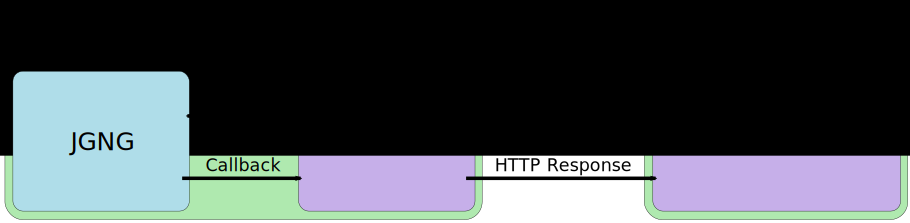
\includegraphics[width=\textwidth]{../figures/client-server.pdf}
        \caption{Übersicht Komponenten}
    \end{figure}
\end{frame}
\begin{frame}
    \frametitle{Anforderungen an die API}
    \begin{itemize}
        \item Auswahl des Algorithmus, zum Trainieren des neuronalen Netzes
        \item Einstellung aller Parameter des Algorithmus
        \item Auswahl eines Datensatzes, zum Trainieren des neuronalen Netzes
        \item Festlegung der Anzahl an Durchläufen für eine Trainingseinheit
        \item Bereitstellung der topologischen Daten des neuronalen Netzes, die der Algorithmus generiert hat
        \item Paralleles Trainieren mehrerer neuronaler Netze
    \end{itemize}
\end{frame}
\begin{frame}
    \frametitle{Anforderungen an die Webanwendung}
    \begin{itemize}
        \item Nutzung der Funktionalität der API
        \item Übersichtliche Darstellung des Trainingsprozesses des neuronalen Netzes
        \item Benutzerfreundliche Möglichkeit zur Parametrisierung des Algorithmus
    \end{itemize}
\end{frame}


\chapter{Grundlagen}
\section{Growing Neural Gas}
\todo[inline, color=green!40]{Growing Neural Gas erklären.}%
\section{Hadoop}
\todo[inline, color=red!40]{Hadoop kurz erklären?}%
\section{REST und JSON}
\todo[inline, color=green!40]{Was ist REST? Was ist JSON?}%
\section{JGNG}
\todo[inline, color=red!40]{Zusammenhang Hadoop und GNG? Kurz!}%


\chapter{REST API des JGNG}
\section{Vorbetrachtung}
\todo[inline, color=green!40]{Anforderungen genau beschreiben. Welche Möglichkeiten gibt es diese zu lösen?}%
\section{Umsetzung}
\todo[inline, color=green!40]{Wie habe ich das gelöst?}%
\section{Zusammenfassung}
\todo[inline, color=red!40]{Kurze Zusammenfassung?}%


\chapter{Webfrontend}
\section{Vorbetrachtung}
\todo[inline, color=green!40]{Anforderungen genau beschreiben. Welche Möglichkeiten gibt es diese zu lösen?}%
\section{Umsetzung}
\todo[inline, color=green!40]{Wie habe ich das gelöst?}%
\section{Zusammenfassung}
\todo[inline, color=red!40]{Kurze Zusammenfassung?}%


\todo[inline, color=red!40]{Zusammenfassungen als extra Kapitel?}%

\chapter{Bewertung und Ausblick}
\section{Bewertung}
\todo[inline, color=green!40]{Wie bewerte ich meine Arbeit. Was ist gut, was weniger? Ziele erreicht?}%
\section{Ausblick}
\todo[inline, color=green!40]{Wie geht es weiter? Was kann man verändern? Was ist offen geblieben?}%



\nocite{*}
\bibliography{literatur}

%\cleardoublepage
%\begingroup
\vspace*{\fill}

\centerline{\textbf{\Large Danksagung}}

\bigskip

Text

\vspace*{\fill}
\endgroup

\pagestyle{empty}
%\cleardoublepage
%\centerline{\textbf{\Large Selbstständigkeitserklärung}}

\bigskip

Ich erkläre gegenüber der Technischen Universität Chemnitz, dass ich die
vorliegende Bachelorarbeit selbstständig und ohne Benutzung anderer als der
angegebenen Quellen und Hilfsmittel angefertigt habe.

Die vorliegende Arbeit ist frei von Plagiaten. Alle Ausführungen, die wörtlich
oder inhaltlich aus anderen Schriften entnommen sind, habe ich als solche
kenntlich gemacht.

Diese Arbeit wurde in gleicher oder ähnlicher Form noch bei keinem anderen
Prüfer als Prüfungsleistung eingereicht und ist auch noch nicht veröffentlicht.

\vspace*{8ex}

\begin{flushright}
\begin{minipage}{5cm}
\footnotesize
\vbox{\hbox to \hsize{\dotfill}\hbox{\hspace{1em}Tobias Gall}}
\end{minipage}
\end{flushright}

\end{document}
